%!Tex Root=**/main.tex
\subsection{Feature-3DGS}
\begin{Frame}{Key Insights}
	\begin{figure}[htbp]
		\begin{annotatedFigureEnv}
			{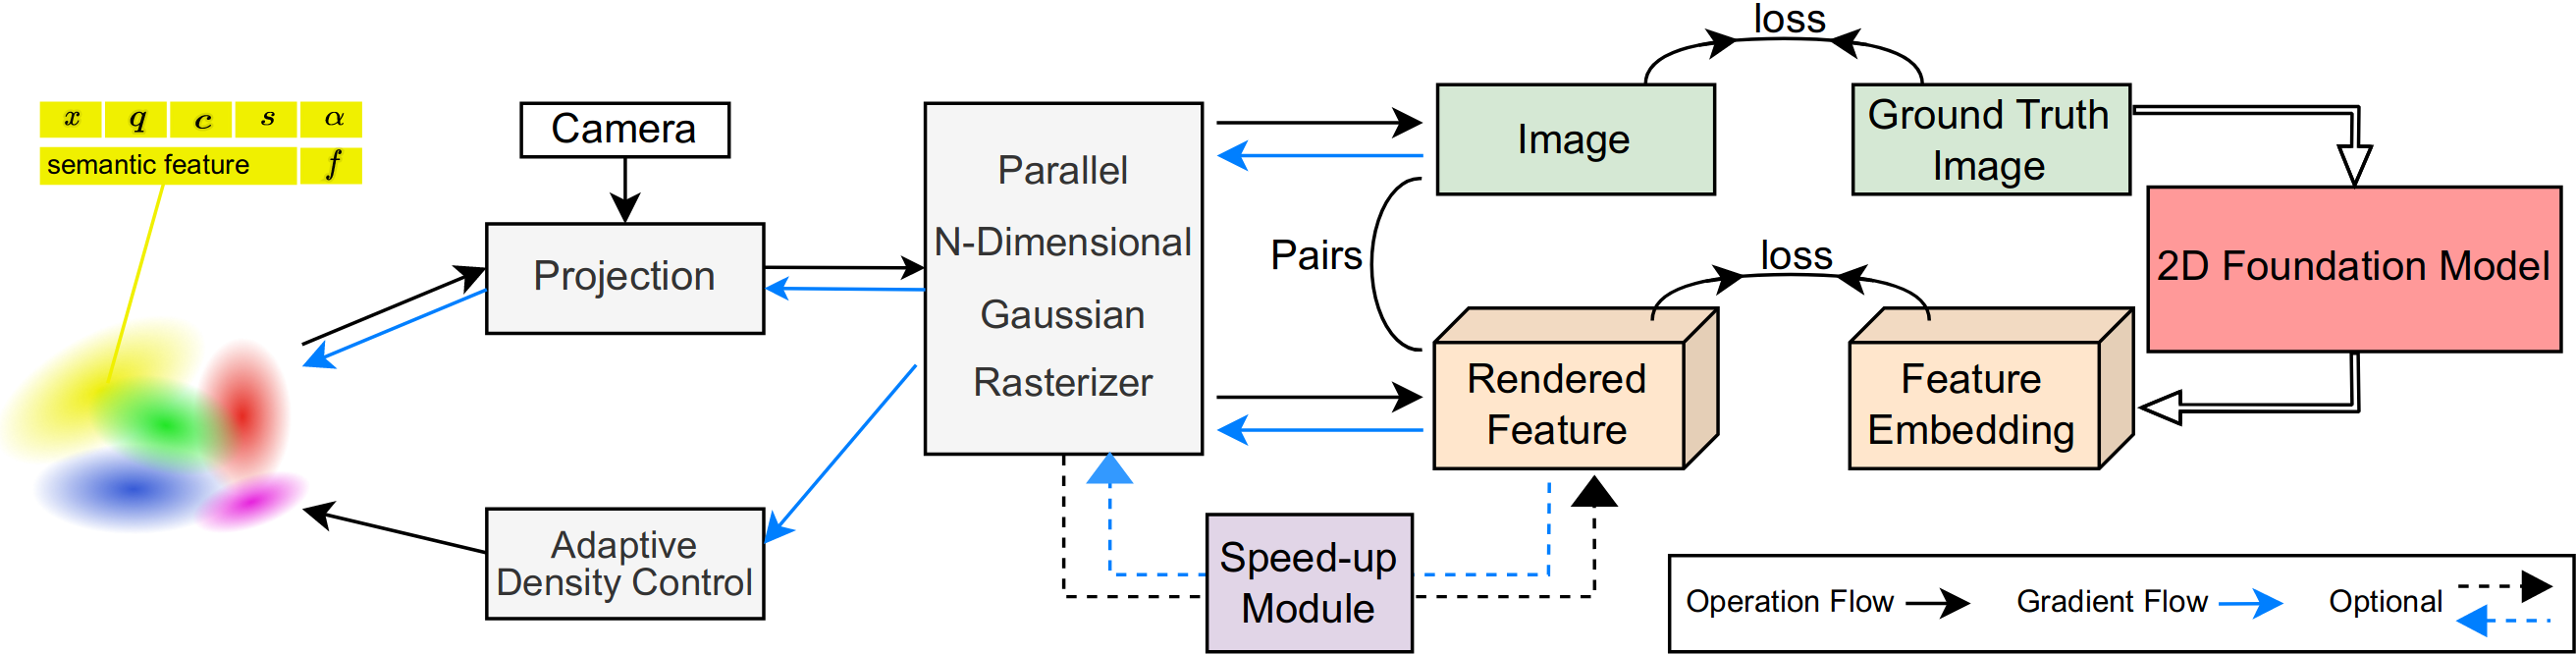
\includegraphics[width=0.85\linewidth]{feature-3dgs-overview.png}}
			\only<1|handout:1>{\annotatedFigure{0,0.7}{0.15,0.78}{1}{0,0.74}}
			\only<1|handout:1>{\annotatedFigure{0.55,0.25}{1,0.72}{1}{0.55,0.72}}
			\only<2->{\annotatedFigure{0.45,-0.05}{0.57,0.25}{2}{0.45,0.25}}
		\end{annotatedFigureEnv}
		\caption{Overview of Feature 3DGS}
	\end{figure}
	\vspace*{\fill}
	\begin{enumerate}
		\setlength{\itemsep}{1.5ex}
		\item<1-> \alert<1>{Semantic Rendering Pipeline}
			\vspace*{1.5ex}
			\par Differentiable rendering of Gaussian-wise latent semantic features.
		\item<2-> \alert<2>{Speed-up module}
			\vspace*{1.5ex}
			\par Dimensionality Alignment.
	\end{enumerate}
	\blfootnote{\href{http://arxiv.org/abs/2312.03203}{(CVPR Highlight, 2024) Feature 3DGS: Supercharging 3D Gaussian Splatting to Enable Distilled Feature Fields}}
\end{Frame}

\begin{Frame}{Semantic Rendering Pipeline}
	\par To render semantic embeddings, i.e.
	\begin{figure}[htbp]
		\vspace*{-2em}
		\centering
		\resetcolorseries[4]{marknode-color-series}
		\resetcolorseries[4]{annotation-color-series}
		\begin{equation}
			\mathbb{R}^{
			\alt<2->{\tikzmarknode{n0}{\colorbox{marknode-color-series!![0]}{\scriptsize \(N\)}}}{N}
			\times
			\alt<3->{\tikzmarknode{n1}{\colorbox{marknode-color-series!![1]}{\scriptsize \(D\)}}}{D}
			}
			\mapsto \mathbb{R}^{
			\alt<4->{\tikzmarknode{n2}{\colorbox{marknode-color-series!![2]}{\scriptsize \(H\)}}}{H}
			\times
			\alt<5->{\tikzmarknode{n3}{\colorbox{marknode-color-series!![3]}{\scriptsize \(W\)}}}{W}
			\times
			D
			}
		\end{equation}
		\begin{annotatedEquationEnv}
			\only<2->{\annotatedEquation{colorseries}{n0}{south}{0em}{-0.5em}{north east}{annotation-color-series}{number of 3D Gaussians}{west}}
			\only<3->{\annotatedEquation{colorseries}{n1}{south}{0em}{-2.0em}{north east}{annotation-color-series}{dimension of semantic embedding}{west}}
			\only<4->{\annotatedEquation{colorseries}{n2}{south}{0em}{-2.0em}{north west}{annotation-color-series}{image height}{east}}
			\only<5->{\annotatedEquation{colorseries}{n3}{south}{0em}{-0.5em}{north west}{annotation-color-series}{image width}{east}}
		\end{annotatedEquationEnv}
	\end{figure}
	\vspace*{\fill}
	\begin{minipage}[c]{0.35\linewidth}
		\definecolor{feature-3dgs-blue}{HTML}{007FFF}
		\visible<6->{\par 5 things,}
		\vspace*{1.5ex}
		\begin{enumerate}[<+(6)-|alert@.>]
			\setlength{\itemsep}{1.5ex}
			\item representation
			\item projection
			\item blending
			\item rasterization
			\item \textcolor{feature-3dgs-blue}{inverse rendering}
		\end{enumerate}
	\end{minipage}
	\begin{minipage}[c]{0.60\linewidth}
		\centering
		\begin{onlyenv}<6->
			\adjustbox{trim={.01\width} {.01\height} {.5\width} {.1\height}, clip}{
				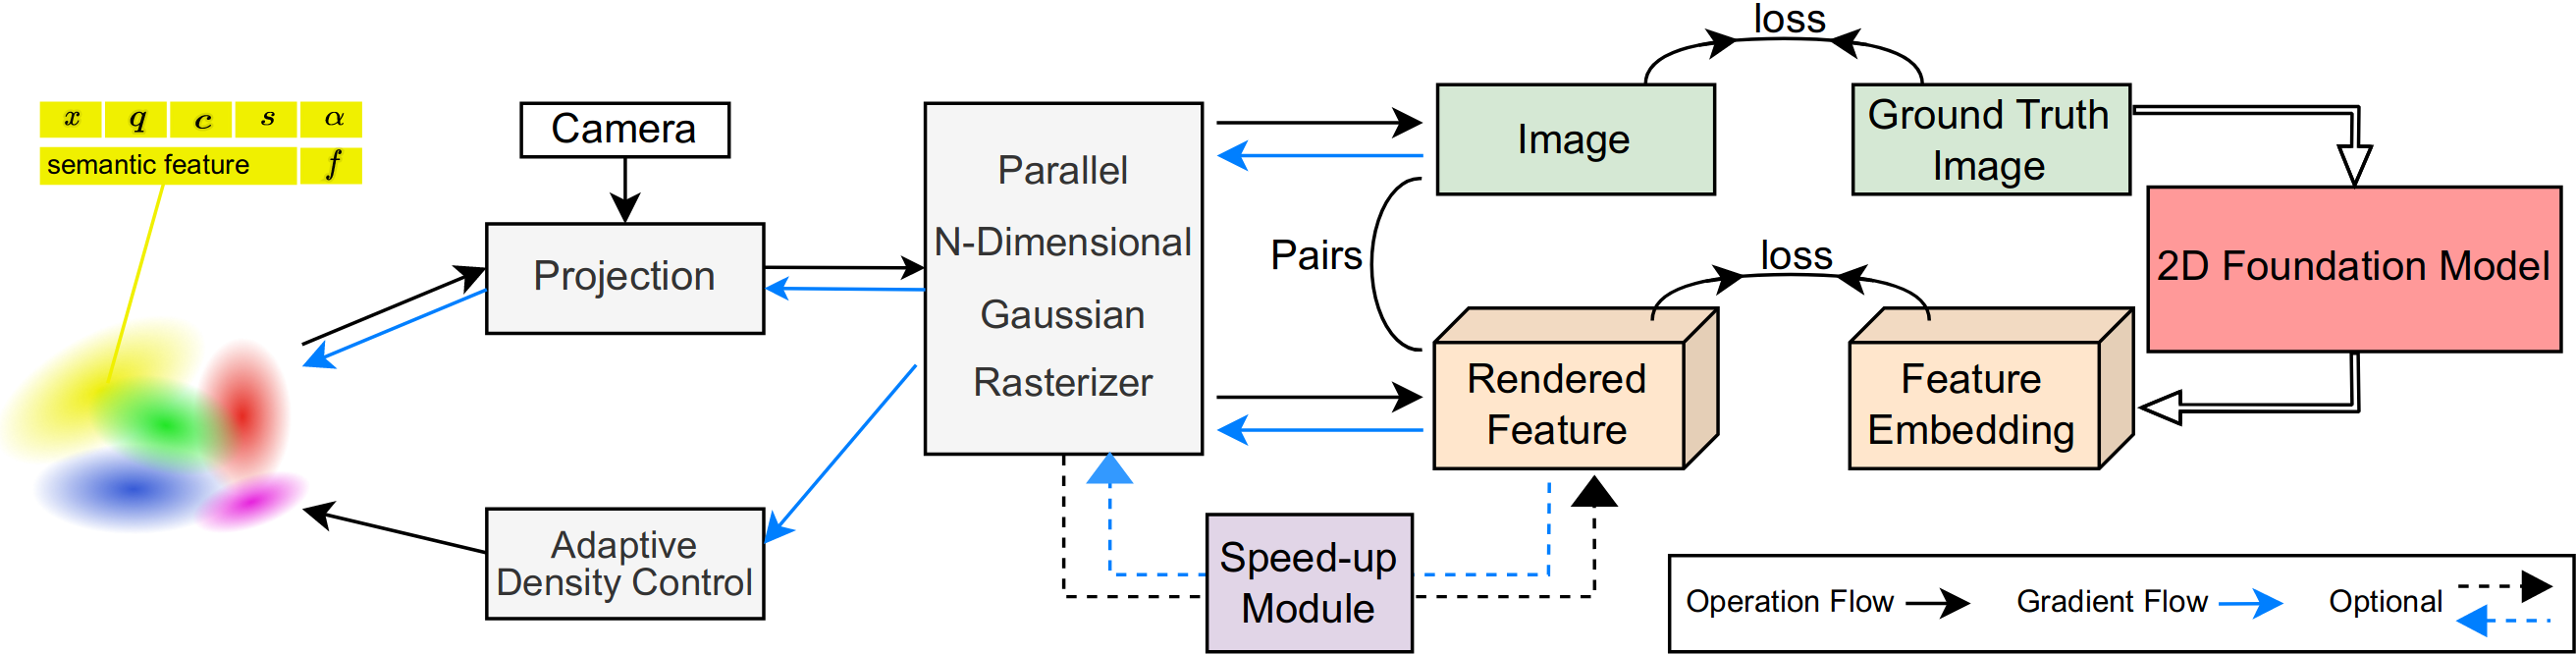
\includegraphics[width=1.5\linewidth]{feature-3dgs-overview.png}
			}
		\end{onlyenv}
	\end{minipage}
	\blfootnote{\href{http://arxiv.org/abs/2312.03203}{(CVPR Highlight, 2024) Feature 3DGS: Supercharging 3D Gaussian Splatting to Enable Distilled Feature Fields}}
\end{Frame}

\begin{Frame}{Semantic Rendering Pipeline \romannum{1}}
	\vspace*{-7em}
	\begin{minipage}[t]{0.70\linewidth}
		\par \alert{Representation}: 3D Gaussian augmented with a latent embedding.
	\end{minipage}
	% \begin{minipage}[t]{0.25\linewidth}
	% 	\centering
	% 	\adjustbox{trim={.01\width} {.01\height} {.85\width} {.01\height}, clip}{
	% 		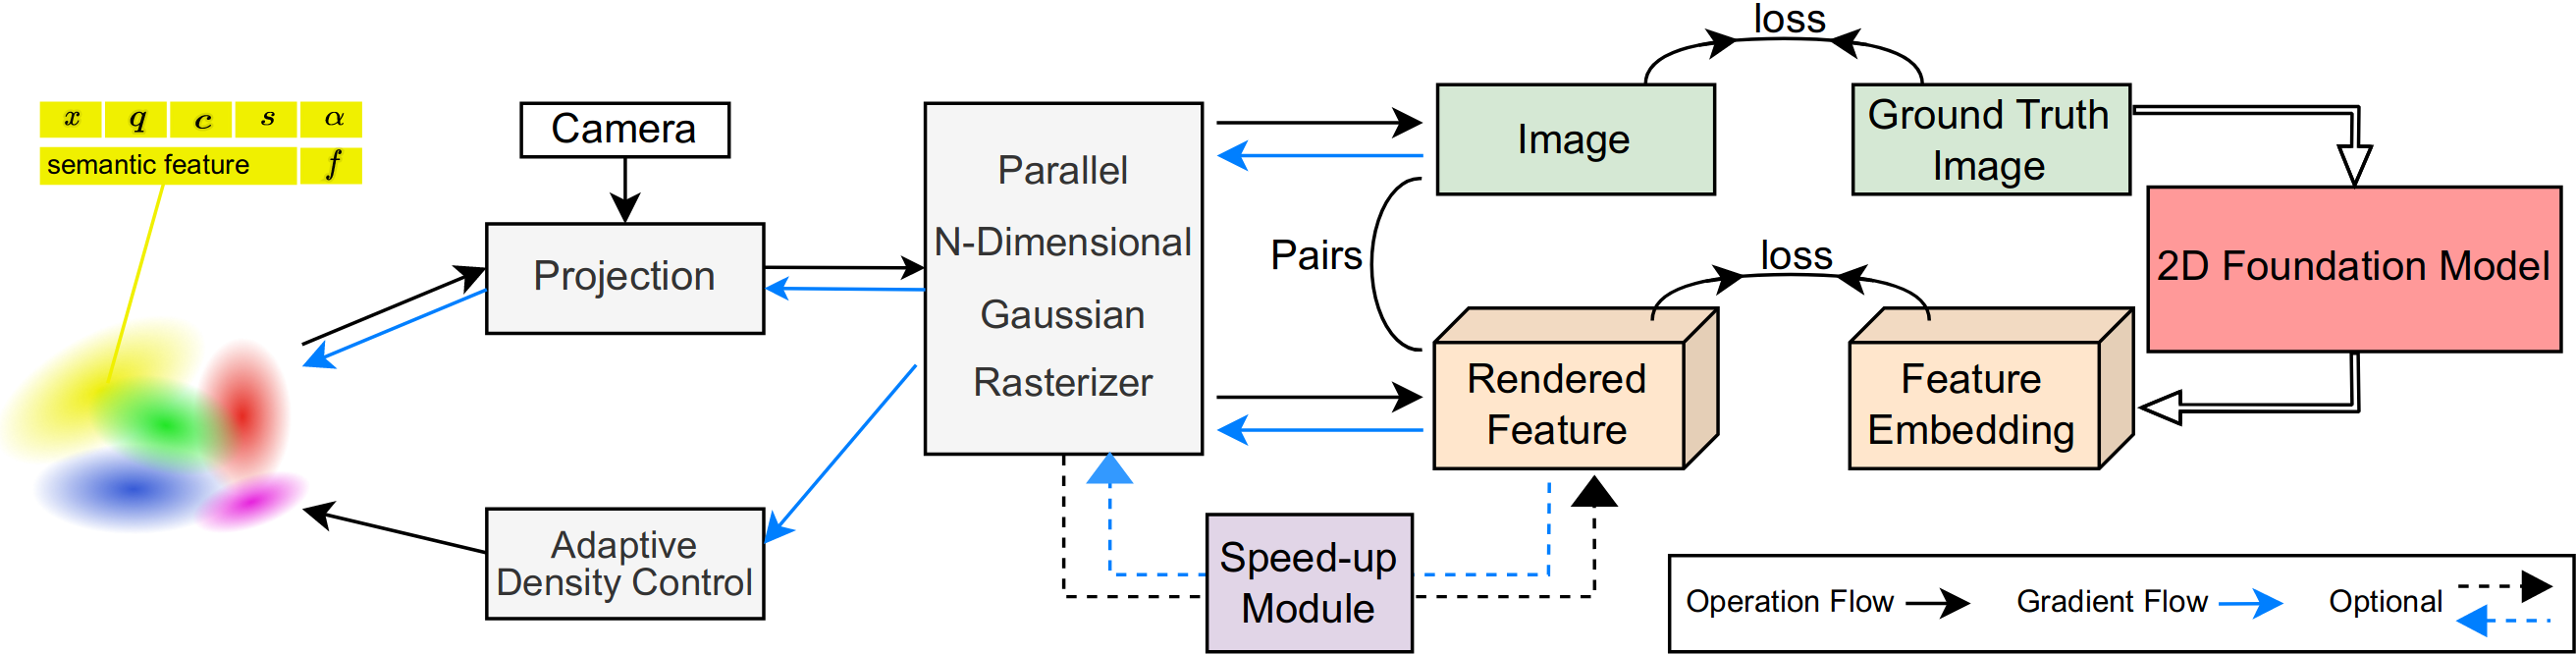
\includegraphics[width=3\linewidth]{feature-3dgs-overview.png}
	% 	}
	% \end{minipage}
	\begin{figure}[htbp]
		\centering
		\resetcolorseries[8]{marknode-color-series}
		\resetcolorseries[8]{annotation-color-series}
		\begin{equation}
			\alt<2-|handout:1>{\tikzmarknode{n0}{\colorbox{marknode-color-series!![0]}{\(\mathcal{G}\)}}}{\mathcal{G}}
			_{
			\alt<3-|handout:1>{\tikzmarknode{n1}{\colorbox{marknode-color-series!![1]}{\scriptsize \(i\)}}}{i}
			}
			=
			\left\{
			\alt<4-|handout:1>{\tikzmarknode{n2}{\colorbox{marknode-color-series!![2]}{\(\mathbf{x}\)},}}{\mathbf{x},}
			\alt<5-|handout:1>{\tikzmarknode{n3}{\colorbox{marknode-color-series!![3]}{\(\mathbf{q}\)},}}{\mathbf{q},}
			\alt<6-|handout:1>{\tikzmarknode{n4}{\colorbox{marknode-color-series!![4]}{\(\mathbf{s}\)},}}{\mathbf{s},}
			\alt<7-|handout:1>{\tikzmarknode{n5}{\colorbox{marknode-color-series!![5]}{\(\alpha\)},}}{\alpha,}
			\alt<8-|handout:1>{\tikzmarknode{n6}{\colorbox{marknode-color-series!![6]}{\(\mathbf{c}\)},}}{\mathbf{c},}
			\alt<9-|handout:1>{\tikzmarknode{n7}{\colorbox{marknode-color-series!![7]}{\(\mathbf{f}\)},}}{\mathbf{f}}
			\right\}
		\end{equation}
		\begin{annotatedEquationEnv}
			\only<2-|handout:1>{\annotatedEquation{colorseries}{n0}{south}{0em}{-0.5em}{north east}{annotation-color-series}{optimizable attributes of a 3D Gaussian}{west}}
			\only<3-|handout:1>{\annotatedEquation{colorseries}{n1}{south}{0em}{-2em}{north east}{annotation-color-series}{\(\in \mathbb{N}\), index of 3D Gaussian}{west}}
			\only<4-|handout:1>{\annotatedEquation{colorseries}{n2}{south}{0em}{-8em}{north west}{annotation-color-series}{\(\in \mathbb{R}^{3}\), position}{east}}
			\only<5-|handout:1>{\annotatedEquation{colorseries}{n3}{south}{0em}{-6.5em}{north west}{annotation-color-series}{\(\in \mathrm{SO}(3)\), rotation}{east}}
			\only<6-|handout:1>{\annotatedEquation{colorseries}{n4}{south}{0em}{-5em}{north west}{annotation-color-series}{\(\in \mathbb{R}^{3}\), scale}{east}}
			\only<7-|handout:1>{\annotatedEquation{colorseries}{n5}{south}{0em}{-3.5em}{north west}{annotation-color-series}{\(\in [0,1]\), opacity}{east}}
			\only<8-|handout:1>{\annotatedEquation{colorseries}{n6}{south}{0em}{-2em}{north west}{annotation-color-series}{\(\in \mathbb{R}^{3n}\), color}{east}}
			\only<9-|handout:1>{\annotatedEquation{colorseries}{n7}{south}{0em}{-0.5em}{north west}{annotation-color-series}{\bf \(\in \mathbb{R}^{3}\), semantic feature}{east}}
		\end{annotatedEquationEnv}
	\end{figure}
	\blfootnote{\(n\): the maximal order of spherical harmonics to represent a color channel. In practice, \(n=4\).}
	\blfootnote{\href{http://arxiv.org/abs/2312.03203}{(CVPR Highlight, 2024) Feature 3DGS: Supercharging 3D Gaussian Splatting to Enable Distilled Feature Fields}}
\end{Frame}

\begin{Frame}{Semantic Rendering Pipeline \romannum{2}}
	\vspace*{-4em}
	\par \alert{Projection}: from 3D ellipsoids to 2D ellipses.
	\begin{figure}[htbp]
		\centering
		\begin{minipage}[c]{0.35\linewidth}
			\begin{onlyenv}<2->
				\resetcolorseries[4]{marknode-color-series}
				\resetcolorseries[4]{annotation-color-series}
				\begin{align}
					\alt<6->{\tikzmarknode{n3}{\colorbox{marknode-color-series!![3]}{\(\mu_{i}\)}}}{\mu_{i}}
					=
					\alt<5->{\tikzmarknode{n2}{\colorbox{marknode-color-series!![2]}{\(\pi\)}}}{\pi}
					\left(
					\alt<4->{\tikzmarknode{n1}{\colorbox{marknode-color-series!![1]}{\(\mathbf{T}_{cw}\)}}}{\mathbf{T}_{cw}}
					\cdot
					\alt<3->{\tikzmarknode{n0}{\colorbox{marknode-color-series!![0]}{\(\mu_{w}\)}}}{\mu_{w}}
					\right)
				\end{align}
				\begin{annotatedEquationEnv}
					\only<3->{\annotatedEquation{colorseries}{n0}{south}{0em}{-1em}{north west}{annotation-color-series}{\(\in \mathbb{P}^3\), 3D(world) mean}{east}}
					\only<4->{\annotatedEquation{colorseries}{n1}{south}{0em}{-3em}{north west}{annotation-color-series}{\(\in \mathrm{SE}(3)\), camera pose}{east}}
					\only<5->{\annotatedEquation{colorseries}{n2}{south}{0em}{-5em}{north west}{annotation-color-series}{projection}{east}}
					\only<6->{\annotatedEquation{colorseries}{n3}{south}{0}{-7em}{north west}{annotation-color-series}{\(\in \mathbb{P}^2\), 2D(image) mean}{east}}
				\end{annotatedEquationEnv}
			\end{onlyenv}
		\end{minipage}
		\begin{minipage}[c]{0.60\linewidth}
			\begin{onlyenv}<2->
				\resetcolorseries[4]{marknode-color-series}
				\resetcolorseries[4]{annotation-color-series}
				\begin{align}
					\alt<10->{\tikzmarknode{n3}{\colorbox{marknode-color-series!![3]}{\(\Sigma_{i}\)}}}{\Sigma_{i}}
					=
					\alt<9->{\tikzmarknode{n2}{\colorbox{marknode-color-series!![2]}{\(\mathbf{J}_{\pi}\)}}}{\mathbf{J}_{\pi}}
					\alt<8->{\tikzmarknode{n1}{\colorbox{marknode-color-series!![1]}{\(\mathbf{R}_{cw}\)}}}{\mathbf{R}_{cw}}
					\alt<7->{\tikzmarknode{n0}{\colorbox{marknode-color-series!![0]}{\(\Sigma_{w}\)}}}{\Sigma_{w}}  \mathbf{R}_{cw}^{\mathrm{T}} \mathbf{J}_{\pi}^{\mathrm{T}}
				\end{align}
				\begin{annotatedEquationEnv}
					\only<7->{\annotatedEquation{colorseries}{n0}{south}{0em}{-1em}{north west}{annotation-color-series}{\(\in \mathbb{R}^{3\times 3}\), 3D(world) covariance}{east}}
					\only<8->{\annotatedEquation{colorseries}{n1}{south}{0em}{-3em}{north west}{annotation-color-series}{\(\in \mathrm{SO(3)}\), rotation component of \(\mathbf{T}_{cw}\)}{east}}
					\only<9->{\annotatedEquation{colorseries}{n2}{south}{0em}{-5em}{north west}{annotation-color-series}{\(\in \mathbb{R}^{2\times 3}\), Jacobian of the linear approximation of \(\pi\)}{east}}
					\only<10->{\annotatedEquation{colorseries}{n3}{south}{0em}{-7em}{north west}{annotation-color-series}{\(\in \mathbb{R}^{2\times 2}\), 2D(image) covariance}{east}}
				\end{annotatedEquationEnv}
			\end{onlyenv}
		\end{minipage}
	\end{figure}
	\blfootnote{\href{http://arxiv.org/abs/2312.03203}{(CVPR Highlight, 2024) Feature 3DGS: Supercharging 3D Gaussian Splatting to Enable Distilled Feature Fields}}
\end{Frame}
% 
\begin{Frame}{Semantic Rendering Pipeline \romannum{3}}
	\par \alert{Blending}: $\alpha$-blending of semantic embeddings.
	\begin{figure}[htbp]
		\centering
		\resetcolorseries[5]{marknode-color-series}
		\resetcolorseries[5]{annotation-color-series}
		\begin{equation}
			\alt<2->{\tikzmarknode{n0}{\colorbox{marknode-color-series!![0]}{\(\mathbf{f}(h,w)\)}}}{\mathbf{f}(h,w)}
			=
			\sum_{i=1}^{
			\alt<6->{\tikzmarknode{n4}{\colorbox{marknode-color-series!![4]}{\scriptsize \(N\)}}}{N}
			}
			\alt<5->{\tikzmarknode{n3}{\colorbox{marknode-color-series!![3]}{\(T_i\)}}}{T_i}
			\alt<4->{\tikzmarknode{n2}{\colorbox{marknode-color-series!![2]}{\(\alpha_i\)}}}{\alpha_i}
			\alt<3->{\tikzmarknode{n1}{\colorbox{marknode-color-series!![1]}{\(\mathbf{f}_i(h,w)\)}}}{\mathbf{f}_i(h,w)}
			,\quad
			\uncover<5->{T_i = \prod_{j=1}^{i-1} (1-\alpha_j)}
		\end{equation}
		\begin{annotatedEquationEnv}
			\only<2->{\annotatedEquation{colorseries}{n0}{south}{0em}{-0.5em}{north east}{annotation-color-series}{semantic feature on pixel \((h,w)\)}{west}}
			\only<3->{\annotatedEquation{colorseries}{n1}{south}{0em}{-1em}{north west}{annotation-color-series}{semantic feature of \(i\)-th Gaussian on pixel \((h,w)\)}{east}}
			\only<4->{\annotatedEquation{colorseries}{n2}{south}{0em}{-2.5em}{north west}{annotation-color-series}{opacity of \(i\)-th Gaussian}{east}}
			\only<5->{\annotatedEquation{colorseries}{n3}{south}{0em}{-4em}{north west}{annotation-color-series}{background opacity for \(i\)-th Gaussian}{east}}
			\only<6->{\annotatedEquation{colorseries}{n4}{north}{0em}{0.5em}{south west}{annotation-color-series}{number of the \textbf{sorted \& visible} subset of 3D Gaussians}{east}}
		\end{annotatedEquationEnv}
	\end{figure}
	% \begin{minipage}[c]{0.20\linewidth}
	% 	\centering
	% 	\adjustbox{trim={.30\width} {.30\height} {.50\width} {.01\height}, clip}{
	% 		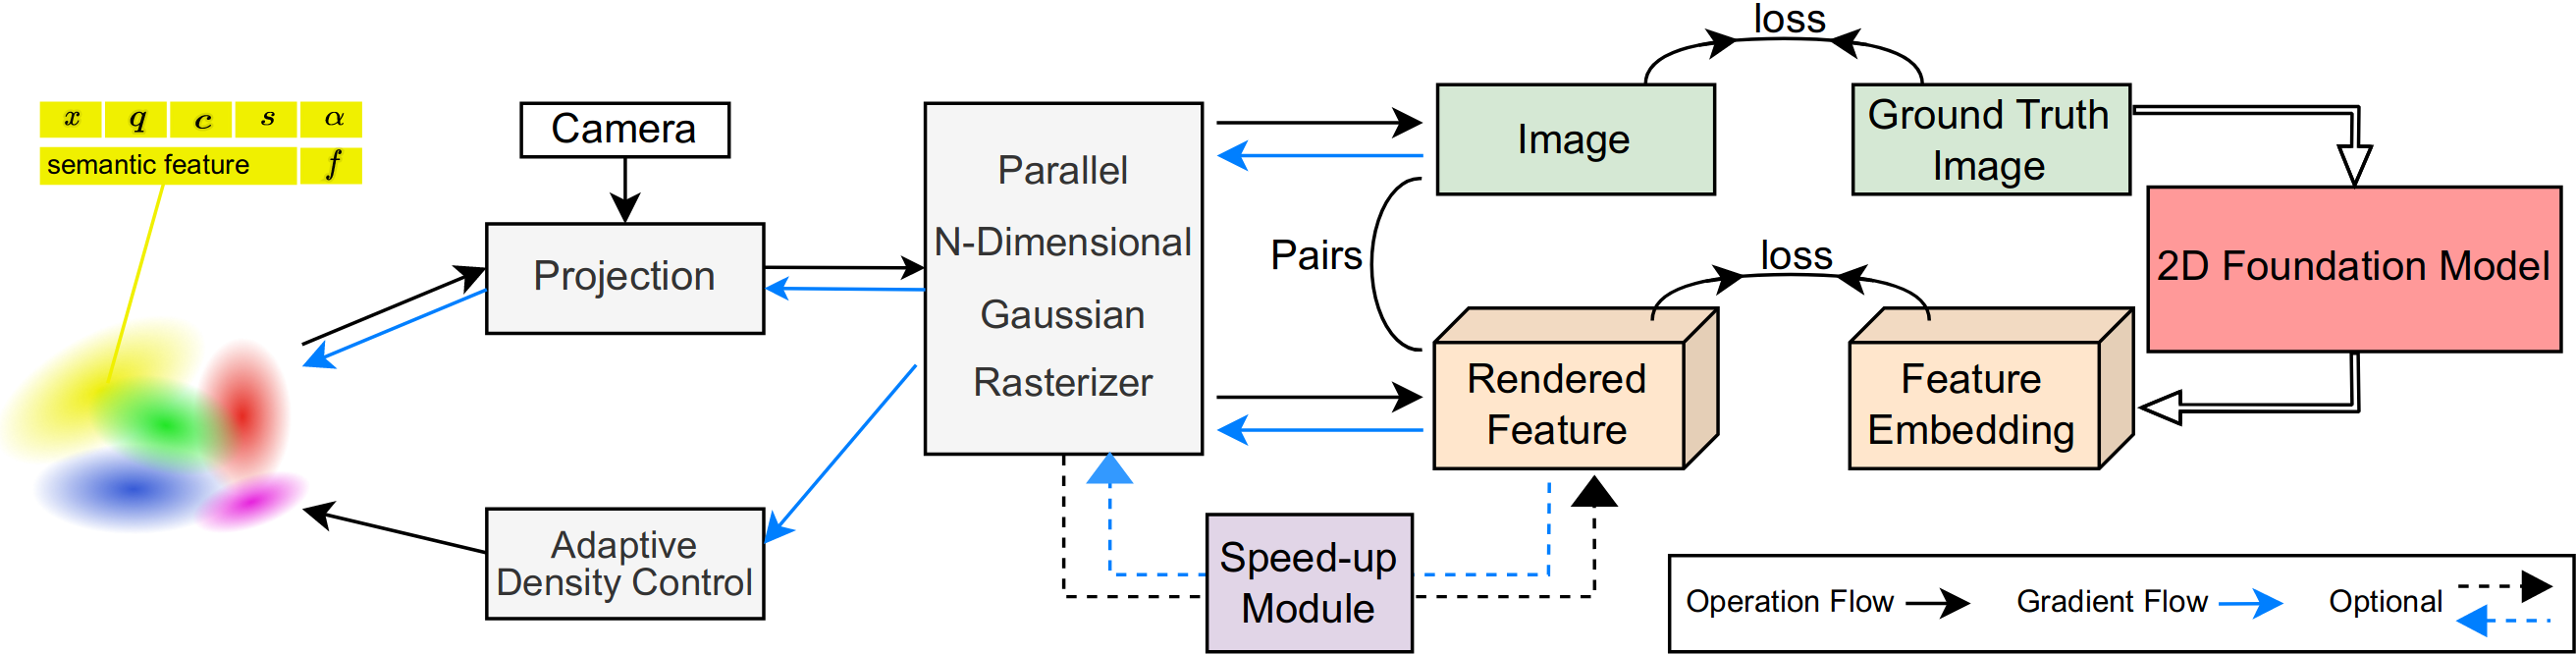
\includegraphics[width=5\linewidth]{feature-3dgs-overview.png}
	% 	}
	% \end{minipage}
	\blfootnote{\href{http://arxiv.org/abs/2312.03203}{(CVPR Highlight, 2024) Feature 3DGS: Supercharging 3D Gaussian Splatting to Enable Distilled Feature Fields}}
\end{Frame}

\begin{Frame}{Semantic Rendering Pipeline \romannum{4}}
	\par \alert{Rasterization}: tiled and implemented in CUDA.
	\vspace*{1.5ex}
	\begin{figure}[htbp]
		\begin{minipage}[c]{0.25\linewidth}
			\centering
			\adjustbox{trim={.30\width} {.30\height} {.50\width} {.01\height}, clip}{
				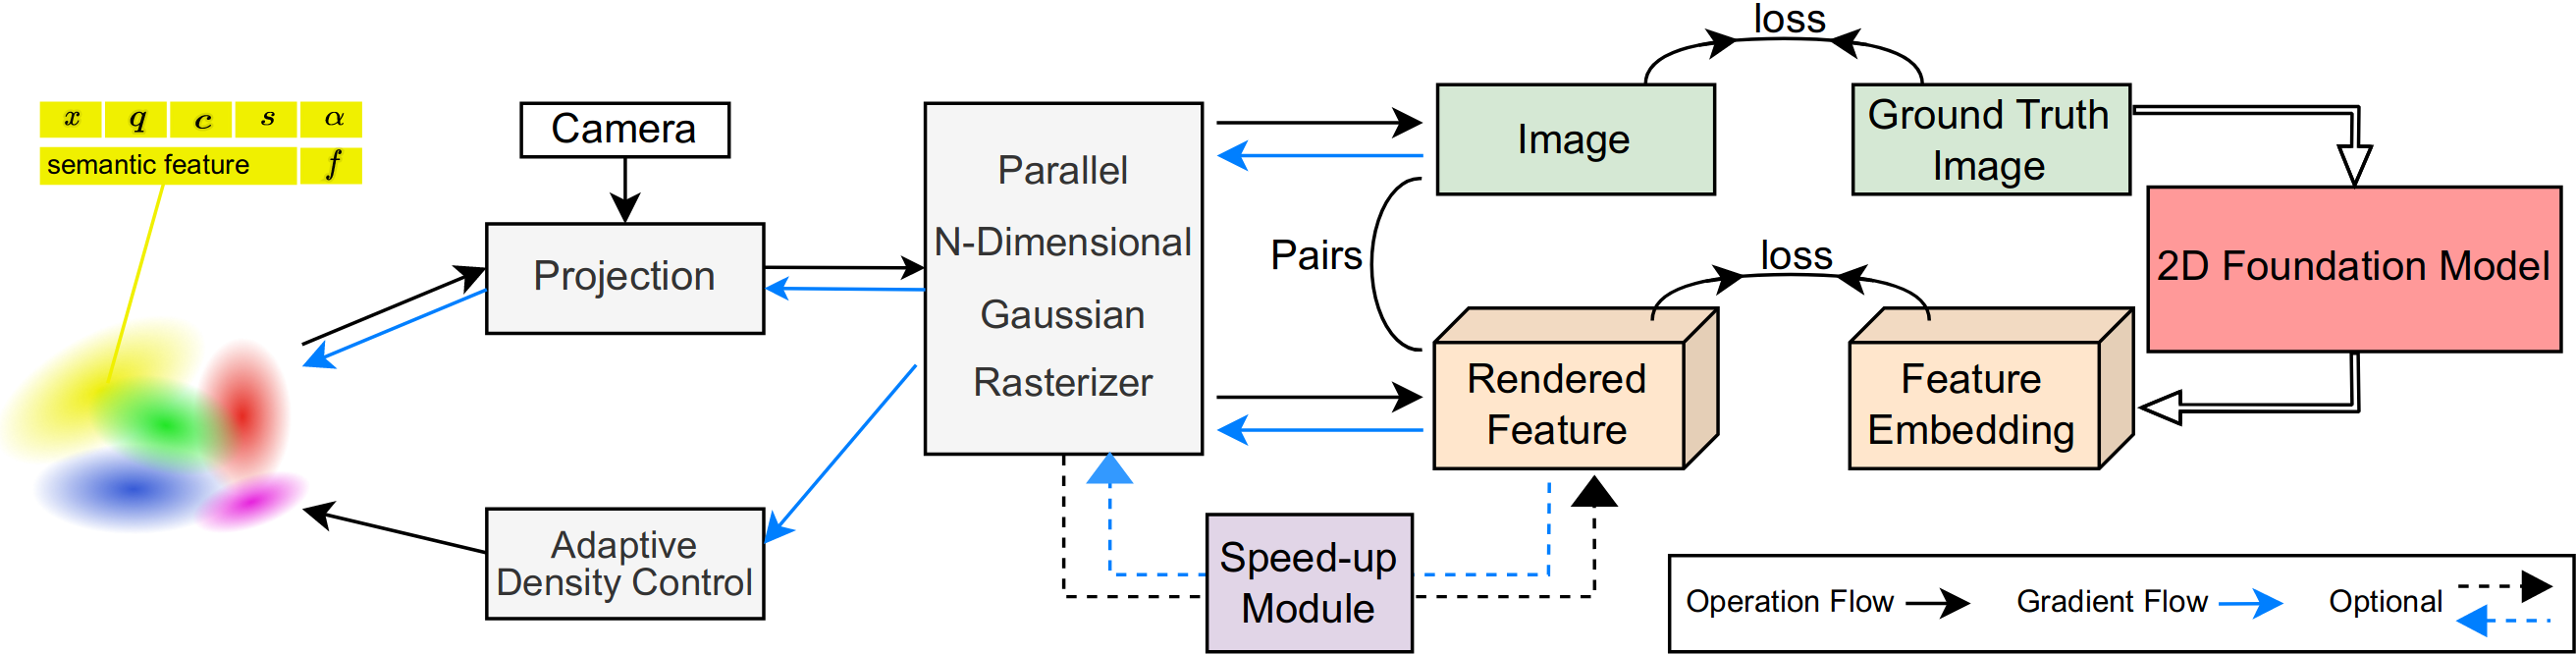
\includegraphics[width=4\linewidth]{feature-3dgs-overview.png}
			}
		\end{minipage}
		\hspace{\fill}
		\begin{minipage}[c]{0.70\linewidth}
			\centering
			\begin{enumerate}[<+(1)->]
				\setlength{\itemsep}{1.5ex}
				\item \alert<.(1)|handout:0>{Divide} the screen space into tiles (CUDA thread blocks).
				\item \alert<.(1)|handout:0>{Group} the Gaussians by view frustum and tile index.
				\item \alert<.(1)|handout:0>{Sort} the Gaussians by front-to-back depth order.
				\item \alert<.(1)|handout:0>{Blend} each pixel within a tile in parallel (CUDA threads).
			\end{enumerate}
		\end{minipage}
	\end{figure}
	\blfootnote{In practice, \(16\times 16\) blocks.}
	\blfootnote{\href{http://arxiv.org/abs/2312.03203}{(CVPR Highlight, 2024) Feature 3DGS: Supercharging 3D Gaussian Splatting to Enable Distilled Feature Fields}}
\end{Frame}

\begin{Frame}{Semantic Rendering Pipeline \romannum{5}}
	\alert<1->{Inverse rendering}: guided by image-wise photometric loss,
	\begin{uncoverenv}<2->
		\begin{figure}[htbp]
			\begin{minipage}[c]{0.25\linewidth}
				\centering
				\adjustbox{trim={.55\width} {.26\height} {.18\width} {.01\height}, clip}{
					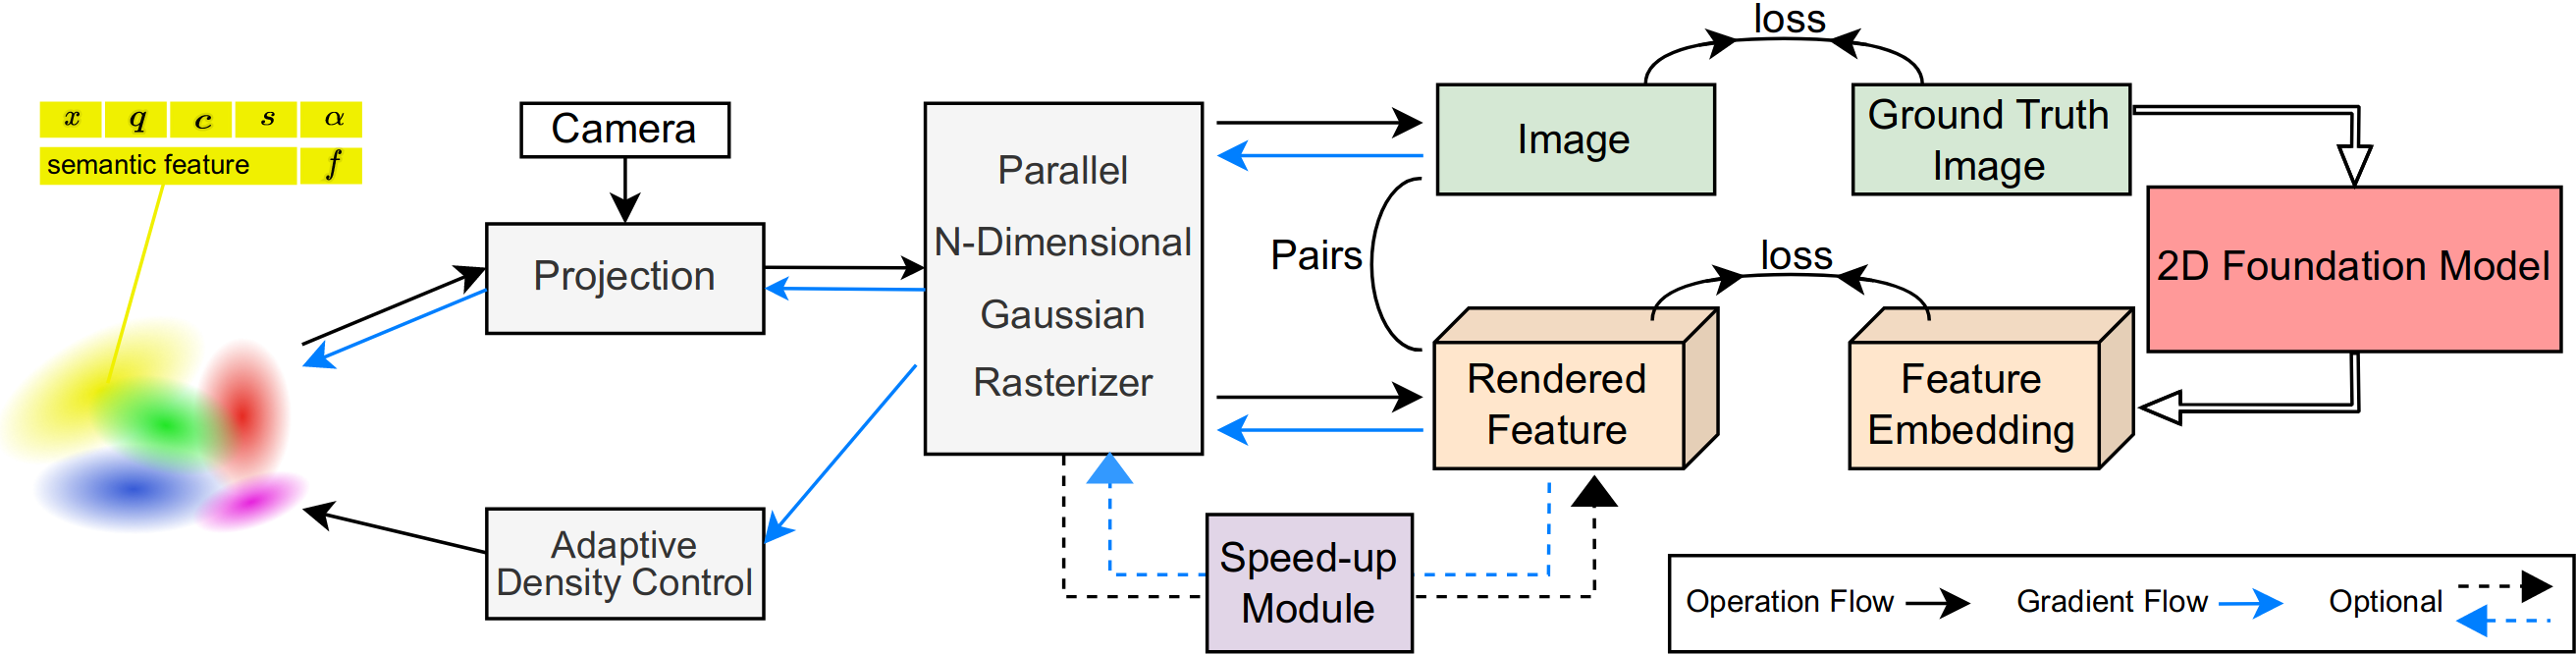
\includegraphics[width=3\linewidth]{feature-3dgs-overview.png}
				}
			\end{minipage}
			\begin{minipage}[c]{0.65\linewidth}
				\centering
				\begin{equation}
					\mathcal{L} = \mathcal{L}_{appearance} + \gamma \mathcal{L}_{semantics}
				\end{equation}
			\end{minipage}
		\end{figure}
	\end{uncoverenv}
	\begin{figure}[htbp]
		\resetcolorseries[2]{marknode-color-series}
		\resetcolorseries[2]{annotation-color-series}
		\visible<3->{
			\begin{alignat}{2}
				 & \mathcal{L}_{appearance} &  & = (1-\lambda) \mathcal{L}_{1} \left(
				\alt<4->{\tikzmarknode{n0}{\colorbox{marknode-color-series!![0]}{\(\mathbf{C}\)}}}{\mathbf{C}}
				,
				\alt<4->{\tikzmarknode{n1}{\colorbox{marknode-color-series!![0]}{\(\hat{\mathbf{C}}\)}}}{\hat{\mathbf{C}}}
				\right) + \lambda \mathcal{L}_{D-SSIM}\left(\mathbf{C}, \hat{\mathbf{C}}\right) \\
				\visible<5->{
				 & \mathcal{L}_{semantics}  &  & = \mathcal{L}_{1} \left(
					\alt<6->{\tikzmarknode{n2}{\colorbox{marknode-color-series!![1]}{\(\mathbf{F}\)}}}{\mathbf{F}}
					,\alt<6->{\tikzmarknode{n3}{\colorbox{marknode-color-series!![1]}{\(\hat{\mathbf{F}}\)}}}{\hat{\mathbf{F}}}
					\right) = \sum_{h=1}^{H} \sum_{w=1}^{W} \Vert \mathbf{f}{(h, w)}-\hat{\mathbf{f}}{(h, w)} \Vert_1
				}
			\end{alignat}
		}
		\begin{annotatedEquationEnv}
			\only<4->{\annotatedEquation{color}{n0}{north}{0em}{1.2em}{south east}{annotation-color-series!!}{captured RGB image (GT)}{west}}
			\only<4->{\annotatedEquation{color}{n1}{north}{0em}{1em}{south west}{annotation-color-series!!}{rendered RGB image}{east}}
			\textcolor{annotation-color-series!!+}{}%
			\only<6->{\annotatedEquation{color}{n2}{south}{0em}{-1.5em}{north east}{annotation-color-series!!}{inferred semantic feature map}{west}}
			\only<6->{\annotatedEquation{color}{n3}{south}{0em}{-1.5em}{north west}{annotation-color-series!!}{rendered semantic feature map}{east}}
		\end{annotatedEquationEnv}
	\end{figure}
	\blfootnote{In practice, \(\gamma=1, \lambda=0.2\).}
	\blfootnote{\href{http://arxiv.org/abs/2312.03203}{(CVPR Highlight, 2024) Feature 3DGS: Supercharging 3D Gaussian Splatting to Enable Distilled Feature Fields}}
\end{Frame}

\begin{Frame}{Speed-up Module}
	\begin{block}<+->{Motivation}
		\par Too \textbf{inefficient} to embed naively,
		\begin{enumerate}[<+->]
			\setlength{\itemsep}{1.5ex}
			\item \alert<.>{High dimension:} latent features in large foundation models.
			\item \alert<.>{Large quantities:} millions of Gaussians in a scene.
		\end{enumerate}
	\end{block}
	\vspace*{\fill}
	\begin{block}<+->{Solution}
		\begin{enumerate}[<+->]
			\setlength{\itemsep}{1.5ex}
			\item \alert<.>{Compactness:} to embed Gaussians with more compact vectors, \(\dim = D^{\,\prime} < D\).
			\item \alert<.>{Alignment:} to align the dimensionalities using a lightweight decoder.
		\end{enumerate}
	\end{block}
	\blfootnote{\(D = 512\) in CLIP; \(D = 256\) in SAM.}
	\blfootnote{In practice, \(D^{\,\prime} = 128\).}
	\blfootnote{Lightweight decoder: In practice, a \(1\times 1\) convolutional layer or a fully-connected layer.}
	\blfootnote{\href{http://arxiv.org/abs/2312.03203}{(CVPR Highlight, 2024) Feature 3DGS: Supercharging 3D Gaussian Splatting to Enable Distilled Feature Fields}}
\end{Frame}

\begin{Frame}{Limitations}
	\begin{enumerate}[<+->]
		\setlength{\itemsep}{1.5ex}
		\item Inefficiency
		      \vspace*{1.5ex}
		      \begin{itemize}
			      \setlength{\itemsep}{1.5ex}
			      \item ``Speed-up module'' is not enough,
			            \visible<+->{
				            \vspace*{1.5ex}
				            \par \(\dim = 128\) embedding for millions of Gaussians.
			            }
		      \end{itemize}
		      \vspace*{1.5ex}
		\item 3D Inconsistency \& Inaccuracy
		      \vspace*{1.5ex}
		      \begin{itemize}
			      \setlength{\itemsep}{1.5ex}
			      \item 2D foundation models are still 2D.
		      \end{itemize}
	\end{enumerate}
	\blfootnote{\href{http://arxiv.org/abs/2312.03203}{(CVPR Highlight, 2024) Feature 3DGS: Supercharging 3D Gaussian Splatting to Enable Distilled Feature Fields}}
\end{Frame}

